% Source PDF page 239 (printed p. 225)
\subsubsection*{不等式形式线性规划的拉格朗日对偶}
类似地，可以求出不等式形式线性规划
\begin{equation}
\begin{array}{ll}\text{最小化}&c^\T x\\\text{约束为}&Ax\preceq b\end{array}\tag{5.21}
\end{equation}
的拉格朗日对偶问题。拉格朗日函数为
\[
L(x,\lambda)=c^\T x+\lambda^\T(Ax-b)
=-b^\T\lambda+(A^\T\lambda+c)^\T x,
\]
所以对偶函数为
\[
g(\lambda)=\inf_x L(x,\lambda)
=-b^\T\lambda+\inf_x(A^\T\lambda+c)^\T x.
\]
线性函数的下确界为 $-\infty$，唯一例外是它恒为零。因此对偶函数为
\[
g(\lambda)=\begin{cases}
-b^\T\lambda&A^\T\lambda+c=0,\\
-\infty&\text{其他情形}.
\end{cases}
\]
若 $\lambda\succeq0$ 且 $A^\T\lambda+c=0$，则对偶变量 $\lambda$ 对偶可行。

线性规划（5.21）的拉格朗日对偶是在所有 $\lambda\succeq0$ 上最大化 $g$。同样，把对偶可行条件显式列为约束，就可改写为
\begin{equation}
\begin{array}{ll}\text{最大化}&-b^\T\lambda\\
\text{约束为}&A^\T\lambda+c=0\\&\lambda\succeq0,\end{array}\tag{5.22}
\end{equation}
这是一个标准形式的线性规划。

标准形式与不等式形式的线性规划及其对偶之间存在有趣的对称性：标准形式线性规划的对偶是仅含不等式约束的线性规划，反之亦然。还可验证，（5.22）的拉格朗日对偶与原始问题（5.21）等价。

\subsection{弱对偶}
拉格朗日对偶问题的最优值记为 $d^\star$。按定义，它是从拉格朗日对偶函数能得到的 $p^\star$ 的最佳下界。特别地，有简单而重要的不等式
\begin{equation}
d^\star\le p^\star,\tag{5.23}
\end{equation}
即使原问题非凸，这一不等式也成立。该性质称为\emph{弱对偶}。

当 $d^\star,p^\star$ 是无穷值时，弱对偶不等式（5.23）也成立。例如，若原始问题无下界，即 $p^\star=-\infty$，则必有 $d^\star=-\infty$，也就是说拉格朗日对偶问题不可行。反之，若对偶问题无上界，即 $d^\star=\infty$，则必有 $p^\star=\infty$，也就是说原始问题不可行。

% Source PDF page 240 (printed p. 226)
称差值 $p^\star-d^\star$ 为原问题的\emph{最优对偶间隙}，因为它给出原始问题最优值与拉格朗日对偶函数能够提供的最佳（即最大）下界之间的差距。最优对偶间隙总是非负的。

由于对偶问题总是凸的，许多情况下可高效求解出 $d^\star$，因此有时可以利用（5.23）为一个难解问题的最优值求下界。例如，考虑第219页的二划分问题（5.7）。它的对偶问题是半正定规划
\[
\begin{array}{ll}\text{最大化}&-\one^\T\nu\\
\text{约束为}&W+\diag(\nu)\succeq0,\end{array}
\]
变量为 $\nu\in\R^n$。即使 $n$ 相当大，例如 $n=1000$，也能高效求解这个问题。其最优值是二划分问题最优值的下界，而且至少与基于 $\lambda_{\min}(W)$ 的下界（5.8）一样好。

\subsection{强对偶与Slater约束资格}
若等式
\begin{equation}
d^\star=p^\star\tag{5.24}
\end{equation}
成立，即最优对偶间隙为零，则称\emph{强对偶}成立。这意味着从拉格朗日对偶函数能够得到的最佳下界是紧的。

一般而言，强对偶未必成立。不过，若原始问题（5.1）是凸的，即具有形式
\begin{equation}
\begin{array}{ll}\text{最小化}&f_0(x)\\
\text{约束为}&f_i(x)\le0,\quad i=1,\ldots,m\\&Ax=b,\end{array}\tag{5.25}
\end{equation}
其中 $f_0,\ldots,f_m$ 凸，则通常（但并非总是）有强对偶。有许多结果给出除凸性以外还能保证强对偶的条件，这些条件称为\emph{约束资格}。

一个简单的约束资格是\emph{Slater条件}：存在 $x\in\relint D$，使得
\begin{equation}
f_i(x)<0,\quad i=1,\ldots,m,\qquad Ax=b.\tag{5.26}
\end{equation}
这样的点有时称为\emph{严格可行点}，因为不等式约束都严格成立。Slater定理说明，若Slater条件成立（且问题凸），则强对偶成立。

若某些不等式约束函数 $f_i$ 是仿射的，Slater条件还可放宽。若前 $k$ 个约束函数 $f_1,\ldots,f_k$ 仿射，那么只要满足以下较弱条件，强对偶就成立：存在 $x\in\relint D$，满足
\begin{equation}
\begin{gathered}
f_i(x)\le0,\quad i=1,\ldots,k,\qquad
f_i(x)<0,\quad i=k+1,\ldots,m,\\
Ax=b.
\end{gathered}\tag{5.27}
\end{equation}

% Source PDF page 241 (printed p. 227)
换言之，仿射不等式不必严格成立。注意，当约束全为线性等式和不等式，且 $\dom f_0$ 是开集时，放宽的Slater条件（5.27）就简化为可行性。

Slater条件（以及放宽的条件（5.27））不仅蕴含凸问题的强对偶，还蕴含当 $d^\star>-\infty$ 时，对偶最优值能够达到。也就是说，存在对偶可行的 $(\lambda^\star,\nu^\star)$，满足 $g(\lambda^\star,\nu^\star)=d^\star=p^\star$。§5.3.2将证明：当原始问题凸且Slater条件成立时，强对偶成立。

\subsection{例子}
\subsubsection*{线性方程的最小二乘解}
回顾问题（5.5）：
\[
\begin{array}{ll}\text{最小化}&x^\T x\\\text{约束为}&Ax=b.\end{array}
\]
相应对偶问题为
\[
\text{最大化}\quad -(1/4)\nu^\T AA^\T\nu-b^\T\nu,
\]
这是无约束的凹二次最大化问题。

Slater条件仅要求原始问题可行，因此只要 $b\in\mathcal R(A)$，即 $p^\star<\infty$，就有 $p^\star=d^\star$。事实上，这个问题总有强对偶，即使 $p^\star=\infty$ 也如此。当 $b\notin\mathcal R(A)$ 时，存在 $z$ 使 $A^\T z=0$、$b^\T z\ne0$。因此对偶函数沿直线 $\{tz\mid t\in\R\}$ 无上界，从而也有 $d^\star=\infty$。

\subsubsection*{线性规划的拉格朗日对偶}
根据较弱的Slater条件，只要原始问题可行，任意线性规划（标准形式或不等式形式）都有强对偶。对其对偶问题也应用这个结果，可知只要对偶可行，线性规划也有强对偶。因此，线性规划强对偶可能失败的情况只剩一种：原始问题和对偶问题都不可行。这种病态情形确实可能发生，见习题5.23。

\subsubsection*{QCQP的拉格朗日对偶}
考虑二次约束二次规划
\begin{equation}
\begin{array}{ll}\text{最小化}&(1/2)x^\T P_0x+q_0^\T x+r_0\\
\text{约束为}&(1/2)x^\T P_ix+q_i^\T x+r_i\le0,\quad i=1,\ldots,m,\end{array}\tag{5.28}
\end{equation}
其中 $P_0\in\mathbf S_{++}^n$，$P_i\in\mathbf S_+^n$，$i=1,\ldots,m$。拉格朗日函数为
\[
L(x,\lambda)=(1/2)x^\T P(\lambda)x+q(\lambda)^\T x+r(\lambda),
\]
其中
\[
P(\lambda)=P_0+\sum_{i=1}^m\lambda_i P_i,\quad
q(\lambda)=q_0+\sum_{i=1}^m\lambda_i q_i,\quad
r(\lambda)=r_0+\sum_{i=1}^m\lambda_i r_i.
\]

% Source PDF page 242 (printed p. 228)
对于一般的 $\lambda$，可以求出 $g(\lambda)$ 的表达式，但相当复杂。不过，若 $\lambda\succeq0$，则 $P(\lambda)\succ0$，而且
\[
g(\lambda)=\inf_x L(x,\lambda)
=-(1/2)q(\lambda)^\T P(\lambda)^{-1}q(\lambda)+r(\lambda).
\]
因此，对偶问题可写为
\begin{equation}
\begin{array}{ll}\text{最大化}&-(1/2)q(\lambda)^\T P(\lambda)^{-1}q(\lambda)+r(\lambda)\\
\text{约束为}&\lambda\succeq0.\end{array}\tag{5.29}
\end{equation}
Slater条件说明，若二次不等式约束严格可行，即存在 $x$ 满足
\[
(1/2)x^\T P_ix+q_i^\T x+r_i<0,\quad i=1,\ldots,m,
\]
则（5.29）与（5.28）之间强对偶成立。

\subsubsection*{熵最大化}
下一个例子是熵最大化问题（5.13）：
\[
\begin{array}{ll}\text{最小化}&\sum_{i=1}^n x_i\log x_i\\
\text{约束为}&Ax\preceq b\\&\one^\T x=1,\end{array}
\]
定义域为 $D=\R_+^n$。第222页已求得拉格朗日对偶函数；对偶问题为
\begin{equation}
\begin{array}{ll}
\text{最大化}&-b^\T\lambda-\nu-e^{-\nu-1}\sum_{i=1}^n e^{-a_i^\T\lambda}\\
\text{约束为}&\lambda\succeq0,\end{array}\tag{5.30}
\end{equation}
变量为 $\lambda\in\R^m$、$\nu\in\R$。（5.13）的较弱Slater条件说明，若存在满足 $Ax\preceq b$、$\one^\T x=1$ 的 $x\succ0$，则最优对偶间隙为零。

可以对对偶变量 $\nu$ 解析地最大化，从而简化（5.30）。固定 $\lambda$ 后，目标在关于 $\nu$ 的导数为零时取得最大值，即
\[
\nu=\log\left(\sum_{i=1}^n e^{-a_i^\T\lambda}\right)-1.
\]
把这一 $\nu$ 的最优值代回对偶问题，得到
\[
\begin{array}{ll}
\text{最大化}&-b^\T\lambda-\log\left(\sum_{i=1}^n e^{-a_i^\T\lambda}\right)\\
\text{约束为}&\lambda\succeq0,\end{array}
\]
这是带非负约束的几何规划（凸形式）。

\subsubsection*{最小体积覆盖椭球}
考虑问题（5.14）：
\[
\begin{array}{ll}\text{最小化}&\log\det X^{-1}\\
\text{约束为}&a_i^\T Xa_i\le1,\quad i=1,\ldots,m,\end{array}
\]

% Source PDF page 243 (printed p. 229)
其定义域为 $D=\mathbf S_{++}^n$。拉格朗日对偶函数由（5.15）给出，所以对偶问题可表示为
\begin{equation}
\begin{array}{ll}\text{最大化}&
\log\det\left(\sum_{i=1}^m\lambda_i a_i a_i^\T\right)-\one^\T\lambda+n\\
\text{约束为}&\lambda\succeq0,\end{array}\tag{5.31}
\end{equation}
其中约定当 $X\not\succ0$ 时 $\log\det X=-\infty$。

问题（5.14）的较弱Slater条件要求，存在 $X\in\mathbf S_{++}^n$，使 $a_i^\T Xa_i\le1$，$i=1,\ldots,m$。这一条件总是满足，因此（5.14）与对偶问题（5.31）之间总有强对偶。

\subsubsection*{具有强对偶的非凸二次问题}
在少数情况下，非凸问题也有强对偶。一个重要例子是在单位球上最小化非凸二次函数：
\begin{equation}
\begin{array}{ll}\text{最小化}&x^\T Ax+2b^\T x\\
\text{约束为}&x^\T x\le1,\end{array}\tag{5.32}
\end{equation}
其中 $A\in\mathbf S^n$、$A\not\succeq0$、$b\in\R^n$。由于 $A\not\succeq0$，这不是凸问题。它有时称为\emph{信赖域问题}，出现在单位球上最小化一个函数的二阶近似时；假设该近似在这个区域内大致有效。

拉格朗日函数为
\[
L(x,\lambda)=x^\T Ax+2b^\T x+\lambda(x^\T x-1)
=x^\T(A+\lambda I)x+2b^\T x-\lambda,
\]
所以对偶函数为
\[
g(\lambda)=\begin{cases}
-b^\T(A+\lambda I)^\dagger b-\lambda&
A+\lambda I\succeq0,\quad b\in\mathcal R(A+\lambda I),\\
-\infty&\text{其他情形},
\end{cases}
\]
其中 $(A+\lambda I)^\dagger$ 为 $A+\lambda I$ 的伪逆。因此拉格朗日对偶问题为
\begin{equation}
\begin{array}{ll}\text{最大化}&-b^\T(A+\lambda I)^\dagger b-\lambda\\
\text{约束为}&A+\lambda I\succeq0,\quad b\in\mathcal R(A+\lambda I),\end{array}\tag{5.33}
\end{equation}
变量为 $\lambda\in\R$。虽然从这个表达式看不明显，但它确实是凸优化问题。事实上，它容易求解，因为可写为
\[
\begin{array}{ll}\text{最大化}&-\sum_{i=1}^n(q_i^\T b)^2/(\lambda_i+\lambda)-\lambda\\
\text{约束为}&\lambda\ge-\lambda_{\min}(A),\end{array}
\]
其中 $\lambda_i$、$q_i$ 是 $A$ 的特征值和相应（标准正交）特征向量；当 $q_i^\T b=0$ 时，将 $(q_i^\T b)^2/0$ 解释为 $0$，其他情况下解释为 $\infty$。

虽然原问题（5.32）非凸，但它的最优对偶间隙总为零：（5.32）与（5.33）的最优值总相同。事实上，更一般的结论成立：任意目标为二次函数、只有一个二次不等式约束的优化问题，只要Slater条件成立，就有强对偶，见§B.1。

% Source PDF page 244 (printed p. 230)
\subsection{矩阵博弈的混合策略}
本节用强对偶推导零和矩阵博弈的一个基本结果。考虑两位参与者的博弈。参与者1选择（或行动）$k\in\{1,\ldots,n\}$，参与者2选择 $l\in\{1,\ldots,m\}$。随后参与者1向参与者2支付 $P_{kl}$，其中 $P\in\R^{n\times m}$ 为博弈的\emph{支付矩阵}。参与者1的目标是使支付尽可能小，参与者2的目标则是使其尽可能大。

参与者采用\emph{随机化策略}或\emph{混合策略}，即各自按照某个概率分布随机选择，且双方的选择相互独立：
\[
\operatorname{prob}(k=i)=u_i,\quad i=1,\ldots,n,\qquad
\operatorname{prob}(l=i)=v_i,\quad i=1,\ldots,m.
\]
这里 $u,v$ 给出双方选择的概率分布，也就是相应策略。于是参与者1向参与者2的期望支付为
\[
\sum_{k=1}^n\sum_{l=1}^m u_kv_lP_{kl}=u^\T Pv.
\]
参与者1希望选择 $u$ 使 $u^\T Pv$ 最小；参与者2希望选择 $v$ 使其最大。

先从参与者1的角度分析，假设参与者2知道她的策略 $u$（这显然使参与者2占优）。参与者2会选择 $v$ 使 $u^\T Pv$ 最大，得到期望支付
\[
\sup\{u^\T Pv\mid v\succeq0,\ \one^\T v=1\}
=\max_{i=1,\ldots,m}(P^\T u)_i.
\]
参与者1能做的最好选择，就是选取 $u$ 使这一最坏情况下向参与者2的支付最小，即选择求解以下问题的策略：
\begin{equation}
\begin{array}{ll}\text{最小化}&\max_{i=1,\ldots,m}(P^\T u)_i\\
\text{约束为}&u\succeq0,\quad\one^\T u=1,\end{array}\tag{5.34}
\end{equation}
这是分段线性的凸优化问题。以 $p_1^\star$ 记其最优值。它是在参与者2知道参与者1的策略、并采取对自己最有利行动的情况下，参与者1能安排的最小期望支付。

类似地，可以考虑参与者1知道参与者2策略 $v$ 的情形（这使参与者1占优）。此时参与者1选择 $u$ 使 $u^\T Pv$ 最小，得到期望支付
\[
\inf\{u^\T Pv\mid u\succeq0,\ \one^\T u=1\}
=\min_{i=1,\ldots,n}(Pv)_i.
\]
参与者2选择 $v$ 使这一数值最大，即选择求解以下问题的策略：
\begin{equation}
\begin{array}{ll}\text{最大化}&\min_{i=1,\ldots,n}(Pv)_i\\
\text{约束为}&v\succeq0,\quad\one^\T v=1,\end{array}\tag{5.35}
\end{equation}

% Source PDF page 245 (printed p. 231)
这也是凸优化问题，其目标是分段线性（凹）函数。以 $p_2^\star$ 记其最优值。它是在参与者1知道参与者2策略的情况下，参与者2能够保证得到的最大期望支付。

直观上，知道对手策略会带来优势（至少不会有害）；而且容易证明，总有 $p_1^\star\ge p_2^\star$。非负差值 $p_1^\star-p_2^\star$ 可以理解为知道对手策略给参与者带来的优势。

利用对偶，可以得到初看令人意外的结果：$p_1^\star=p_2^\star$。换言之，在采用混合策略的矩阵博弈中，知道对手策略并不带来优势。下面通过说明（5.34）与（5.35）互为拉格朗日对偶、且强对偶成立，来证明这个结果。

先将（5.34）写成线性规划
\[
\begin{array}{ll}\text{最小化}&t\\
\text{约束为}&u\succeq0,\quad\one^\T u=1\\
&P^\T u\preceq t\one,\end{array}
\]
其中引入额外变量 $t\in\R$。对 $P^\T u\preceq t\one$ 引入乘子 $\lambda$，对 $u\succeq0$ 引入 $\mu$，对 $\one^\T u=1$ 引入 $\nu$，得到拉格朗日函数
\[
\begin{aligned}
&t+\lambda^\T(P^\T u-t\one)-\mu^\T u+\nu(1-\one^\T u)\\
&\qquad=\nu+(1-\one^\T\lambda)t+(P\lambda-\nu\one-\mu)^\T u.
\end{aligned}
\]
因此对偶函数为
\[
g(\lambda,\mu,\nu)=\begin{cases}
\nu&\one^\T\lambda=1,\quad P\lambda-\nu\one=\mu,\\
-\infty&\text{其他情形}.
\end{cases}
\]
于是对偶问题为
\[
\begin{array}{ll}\text{最大化}&\nu\\
\text{约束为}&\lambda\succeq0,\quad\one^\T\lambda=1,\quad\mu\succeq0\\
&P\lambda-\nu\one=\mu.\end{array}
\]
消去 $\mu$，得到（5.34）的拉格朗日对偶
\[
\begin{array}{ll}\text{最大化}&\nu\\
\text{约束为}&\lambda\succeq0,\quad\one^\T\lambda=1\\
&P\lambda\succeq\nu\one,\end{array}
\]
变量为 $\lambda,\nu$。它显然与（5.35）等价。由于这些线性规划可行，强对偶成立；（5.34）与（5.35）的最优值相等。

% Source PDF page 246 (printed p. 232)
\section{几何解释}
\subsection{通过值集解释弱对偶与强对偶}
利用集合
\begin{equation}
\begin{split}
\mathcal G=\{&(f_1(x),\ldots,f_m(x),h_1(x),\ldots,h_p(x),f_0(x))\\
&\in\R^m\times\R^p\times\R\mid x\in D\},
\end{split}\tag{5.36}
\end{equation}
可以给对偶函数一个简单的几何解释。$\mathcal G$ 是约束函数和目标函数所取值组成的集合。问题（5.1）的最优值容易用 $\mathcal G$ 写成
\[
p^\star=\inf\{t\mid(u,v,t)\in\mathcal G,\ u\preceq0,\ v=0\}.
\]
为计算 $(\lambda,\nu)$ 处的对偶函数值，只需在 $(u,v,t)\in\mathcal G$ 上最小化仿射函数
\[
(\lambda,\nu,1)^\T(u,v,t)=\sum_{i=1}^m\lambda_i u_i+\sum_{i=1}^p\nu_i v_i+t,
\]
即
\[
g(\lambda,\nu)=\inf\{(\lambda,\nu,1)^\T(u,v,t)\mid(u,v,t)\in\mathcal G\}.
\]
特别地，若下确界有限，则不等式
\[
(\lambda,\nu,1)^\T(u,v,t)\ge g(\lambda,\nu)
\]
确定 $\mathcal G$ 的一个支撑超平面。有时称它为\emph{非竖直}支撑超平面，因为其法向量的最后一个分量非零。

现在设 $\lambda\succeq0$。显然，当 $u\preceq0$、$v=0$ 时，
$t\ge(\lambda,\nu,1)^\T(u,v,t)$。因此
\[
\begin{aligned}
p^\star&=\inf\{t\mid(u,v,t)\in\mathcal G,\ u\preceq0,\ v=0\}\\
&\ge\inf\{(\lambda,\nu,1)^\T(u,v,t)\mid(u,v,t)\in\mathcal G,\ u\preceq0,\ v=0\}\\
&\ge\inf\{(\lambda,\nu,1)^\T(u,v,t)\mid(u,v,t)\in\mathcal G\}\\
&=g(\lambda,\nu),
\end{aligned}
\]
这就是弱对偶。图5.3和图5.4用一个只有一个不等式约束的简单问题说明这一解释。

\subsubsection*{上图形式的变体}
本节给出基于 $\mathcal G$ 的对偶几何解释的一个变体，它能说明为什么（大多数）凸问题具有强对偶。定义集合 $\mathcal A\subseteq\R^m\times\R^p\times\R$ 为
\begin{equation}
\mathcal A=\mathcal G+\bigl(\R_+^m\times\{0\}\times\R_+\bigr),\tag{5.37}
\end{equation}
更显式地，
\[
\begin{split}
\mathcal A=\{(u,v,t)\mid{}&\exists x\in D,\ f_i(x)\le u_i,\quad i=1,\ldots,m,\\
&h_i(x)=v_i,\quad i=1,\ldots,p,\quad f_0(x)\le t\}.
\end{split}
\]

% Source PDF page 247 (printed p. 233)
\begin{figure}[htbp]\centering
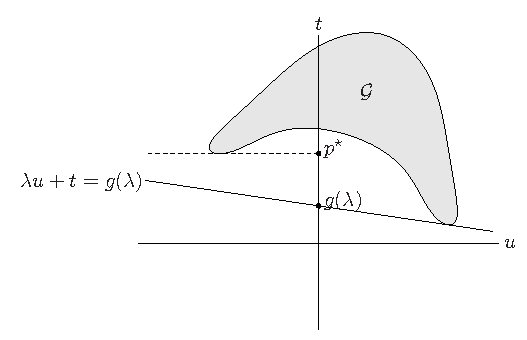
\includegraphics[width=.7\linewidth]{figures/ch05-fig03.pdf}
\caption*{图5.3\quad 对偶函数及下界 $g(\lambda)\le p^\star$ 的几何解释，所示问题含一个（不等式）约束。给定 $\lambda$，在 $\mathcal G=\{(f_1(x),f_0(x))\mid x\in D\}$ 上最小化 $(\lambda,1)^\T(u,t)$，得到斜率为 $-\lambda$ 的支撑超平面。该超平面与 $u=0$ 轴的交点给出 $g(\lambda)$。}
\end{figure}
\begin{figure}[htbp]\centering
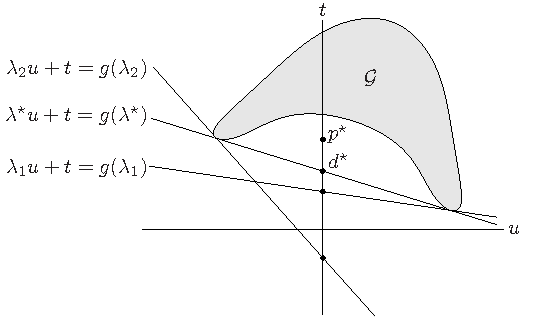
\includegraphics[width=.7\linewidth]{figures/ch05-fig04.pdf}
\caption*{图5.4\quad 三个对偶可行 $\lambda$ 值所对应的支撑超平面，其中包括最优值 $\lambda^\star$。强对偶不成立；最优对偶间隙 $p^\star-d^\star$ 为正。}
\end{figure}

% Source PDF page 248 (printed p. 234)
\begin{figure}[htbp]\centering
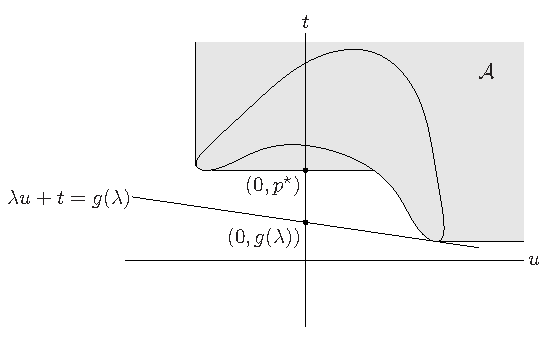
\includegraphics[width=.7\linewidth]{figures/ch05-fig05.pdf}
\caption*{图5.5\quad 对偶函数及下界 $g(\lambda)\le p^\star$ 的几何解释，所示问题含一个（不等式）约束。给定 $\lambda$，在 $\mathcal A=\{(u,t)\mid\exists x\in D,\ f_0(x)\le t,\ f_1(x)\le u\}$ 上最小化 $(\lambda,1)^\T(u,t)$，得到斜率为 $-\lambda$ 的支撑超平面。该超平面与 $u=0$ 轴的交点给出 $g(\lambda)$。}
\end{figure}
可以把 $\mathcal A$ 看作 $\mathcal G$ 的某种上图形式，因为 $\mathcal A$ 包含 $\mathcal G$ 的所有点，也包含“更差”的点，即目标值或不等式约束函数值更大的点。

最优值可用 $\mathcal A$ 表示为
\[
p^\star=\inf\{t\mid(0,0,t)\in\mathcal A\}.
\]
在满足 $\lambda\succeq0$ 的 $(\lambda,\nu)$ 处计算对偶函数值，可在 $\mathcal A$ 上最小化仿射函数 $(\lambda,\nu,1)^\T(u,v,t)$：若 $\lambda\succeq0$，则
\[
g(\lambda,\nu)=\inf\{(\lambda,\nu,1)^\T(u,v,t)\mid(u,v,t)\in\mathcal A\}.
\]
若下确界有限，则
\[
(\lambda,\nu,1)^\T(u,v,t)\ge g(\lambda,\nu)
\]
确定 $\mathcal A$ 的一个非竖直支撑超平面。特别地，因为 $(0,0,p^\star)\in\operatorname{bd}\mathcal A$，所以
\begin{equation}
p^\star=(\lambda,\nu,1)^\T(0,0,p^\star)\ge g(\lambda,\nu),\tag{5.38}
\end{equation}
即弱对偶下界。强对偶成立，当且仅当存在对偶可行的 $(\lambda,\nu)$，使（5.38）取等号；也就是说，在 $\mathcal A$ 的边界点 $(0,0,p^\star)$ 处存在一个非竖直支撑超平面。图5.5说明了这第二种解释。

\subsection{约束资格下强对偶的证明}
本节证明，对凸问题，Slater约束资格保证强对偶（并且对偶最优值能达到）。考虑
